\chapter{The Recipe: Twelve Knobs}

\epi{Preheat the halo to $10^{12}$ solar masses.\\ Season generously with supernovae.\\ Adjust to taste. The taste in question is somebody else's formula.}

\fig[1.0]{plate_recipe_card}{The recipe card. Twelve knobs in four groups, each drawn as a dial. Three of them, in red, ran to the edge of the range I allowed. The card's one honest line: it was tuned to the law, not to the data.}


\section{Why ``fried chicken''?}

The paper this part of the book is built on has a ridiculous title: \emph{ACDM flavored fried chicken version of Galaxy Dynamics}. That is on purpose. It's a research experiment, not a claim. I don't believe the recipes, the halos or the particle readings in it. The point was to work out, carefully and on the record, how a \LCDM\ group \emph{could} reverse-engineer my galaxy law, so that if somebody later presents a tuned match as a derivation, the route is already written down with its knob count attached. ``Fried chicken'' is a nickname with no physics in it. You need a name that nobody will cite as support for anything, and a fast-food name does the job.

The paper went through versions 1.0 to 2.3 between the second and fourth of November 2026, adding a new section every time a new kind of rival recipe was tried. It ran to 48 dated amendments, every one frozen before its numbers were computed, every failed check kept on the record. This chapter and the next four walk through it.

\section{The dish being imitated}

The target is my galaxy law, which Part~IV discusses properly. For now, here it is as a recipe card:
\begin{gather}
\gbar=\frac{g^2}{g+a_0},\\
a_0=\kappa\,c\sqrt{G\rhoDE}=9.36\times10^{-11}\ms,\qquad\kappa=\tfrac12\ \text{(fitted)}.
\end{gather}
Solved for the observed acceleration $g$ given the baryonic one,
\begin{equation}
g_{\rm law}(\gbar)=\frac{\gbar}{2}+\sqrt{\frac{\gbar^2}{4}+\gbar\,a_0}.
\end{equation}
The ingredients are the measured baryons of the SPARC galaxies with fixed mass-to-light ratios, $\Upsilon_{\rm disk}=0.5$ and $\Upsilon_{\rm bul}=0.7$, and no galaxy-by-galaxy adjustment. Four of the 175 galaxies have too few usable points, which leaves 171 galaxies and 3373 points.

\begin{honestbox}
The target is the \emph{law's} curve on each galaxy's own baryons, not the observed rotation curve. This is an imitation contest: can \LCDM's knobs make halos that reproduce the formula? It isn't a contest about which fits the data better. On the observed curves, at these fixed $\Upsilon$, the law's own rms is $0.1951\dex$. Hold onto that number; it comes back with a surprise at the end of the chapter.
\end{honestbox}

\section{How a recipe makes an acceleration}

Every \LCDM\ recipe in the kitchen works the same way. Given a galaxy's baryons, it builds a dark-matter mass profile $M_{\rm DM}(r)$ from its knobs, then adds the halo's pull to the baryons':
\begin{equation}
g_{\rm model}(r)=\gbar(r)+\frac{G\,M_{\rm DM}(r)}{r^2}.
\end{equation}
Compare $g_{\rm model}$ to $g_{\rm law}$ at the same radius, and report three distances (the E1--E3 targets of Chapter~1): pooled rms, the 95th-percentile galaxy, and the worst half-dex bin in $\gbar$.

There's a fourth number, the recipe's own acceleration scale $a$. Fit the law's \emph{form} to the recipe's output, treating $a_0$ as free:
\begin{equation}
a=\arg\min_{a'}\sum_i\Bigl[\log_{10}g_{{\rm model},i}-\log_{10}g_{\rm law}(\gbar{}_{,i};a')\Bigr]^2.
\end{equation}
If the recipe has really learned the law, $a$ should come out at $a_0$.

Before we look at the scores, it helps to see what a distance in dex means on a real rotation curve. Acceleration goes as speed squared, so a gap in acceleration is twice as large, in dex, as the same gap in speed.


\fig{dex_on_curve}{What the scores mean on a rotation curve. The twelve-knob recipe's 0.0415\,dex gap from the law (grey band) is about 5 per cent in speed; the frozen target of 0.02\,dex (red band) is about 2 per cent.}



\section{The menu}

Here is the whole menu, in one table, from the paper's version 2.3. Bold rows pass all three of E1 to E3.

\begin{table}[h]\centering\small
\begin{tabular}{@{}lrrrrr@{}}
\toprule
recipe & knobs & rms & p95 & worst bin & $a/10^{-11}$\\
\midrule
R1 NFW, no tuning & 0 & 0.1419 & 0.2877 & 0.1613 & 15.76\\
R1 tuned, contraction & 4 & 0.0715 & 0.1486 & 0.0441 & 9.12\\
R2 tuned, feedback core & 6 & 0.0721 & 0.1357 & 0.0283 & 8.65\\
R3 thermal, 2 global laws & 2 & 0.2245 & 0.3187 & 0.2261 & 6.06\\
R4 thermal, per galaxy & 342 & 0.0609 & 0.1119 & 0.0260 & 8.97\\
R7 surface density & 9 & 0.0408 & 0.0777 & 0.0413 & 9.21\\
R11 twelve feedback knobs & 12 & 0.0415 & 0.1006 & 0.0221 & 9.33\\
R11b plus $c$ norm, slope & 14 & 0.0275 & 0.0624 & 0.0196 & 9.31\\
R10 six global functions & 42 & 0.0213 & 0.0441 & 0.0216 & 9.30\\
R9 per galaxy, 1$\sigma$ & 1026 & 0.0376 & 0.0711 & 0.0164 & 9.63\\
\textbf{R9 per galaxy, 2$\sigma$} & 1026 & \textbf{0.0152} & \textbf{0.0283} & \textbf{0.0040} & 9.43\\
R8p per galaxy, referee & 684 & 0.0396 & 0.0665 & 0.0148 & 9.72\\
\textbf{R8 per galaxy, wide} & 684 & \textbf{0.0056} & \textbf{0.0130} & \textbf{0.0031} & 9.36\\
\textbf{R6 one empirical function} & 1 & \textbf{0.0075} & \textbf{0.0118} & \textbf{0.0180} & 9.37\\
\textbf{R5 exact shell masses} & 3373 & \textbf{0.0000} & \textbf{0.0000} & \textbf{0.0000} & 9.36\\
\textbf{R12 halo from the formula} & 1 & \textbf{0.0000} & \textbf{0.0000} & \textbf{0.0000} & 9.36\\
\bottomrule
\end{tabular}
\caption{The fried chicken menu: distance to the law in dex. Targets are 0.02, 0.04 and 0.02.}
\end{table}

\begin{figure}[h]
\centering
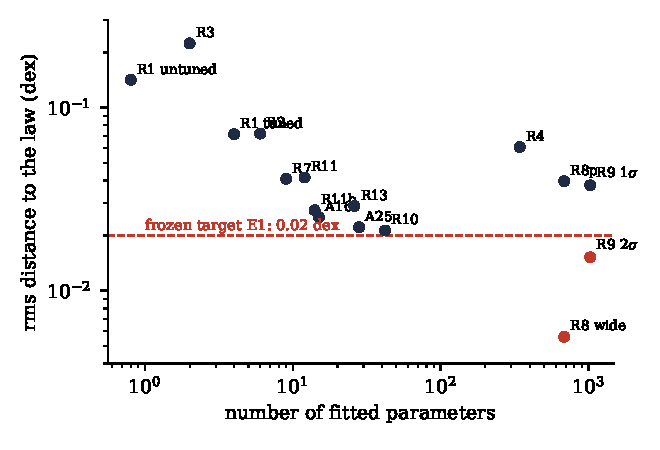
\includegraphics[width=0.92\linewidth]{figures/menu.pdf}
\caption{The knob curve. Each point is a recipe; red points pass the pooled target E1 (dashed). Getting under the line takes either hundreds of per-galaxy knobs or a formula with the law written into it (R5, R6 and R12 aren't plotted; they sit at or near zero by construction).}
\end{figure}

Here is the same menu as a staircase, best recipe at each knob count. Each step down costs more knobs than the last, and the last steps are not recipes at all but the law itself, written as a halo.


\fig{knob_staircase}{Descending the knob staircase. The distance to the law falls as knobs are added, but it crosses the frozen target only with a thousand per-galaxy knobs, or with 3373 knobs that simply restate the law shell by shell.}



We'll come back to the bottom of the menu, where the exact dishes live, in Chapter~5. First, the main course.

\section{Course one: the level comes cheaply}

Start with plain \LCDM: NFW halos, masses from abundance matching, concentrations from the $c(M)$ relation, nothing tuned. That's R1, and it's not close. Its rms distance from the law is $0.1419\dex$, and its acceleration scale is $15.76\times10^{-11}\ms$, about 1.7 times $a_0$. Untouched \LCDM\ halos are too heavy in the middle.

Now turn four knobs: the stellar-to-halo normalisation, the normalisation and mass slope of the concentration relation, and a contraction fraction. The scale drops to $9.12\times10^{-11}$, within 3 per cent of $a_0$.

\begin{honestbox}[The first lesson]
\textbf{Getting the right number from tuned halos is easy, so the number alone proves little.} Four knobs bring \LCDM\ halos to the law's acceleration scale, with the concentration knob sitting at its bound. If you've ever seen ``$\Lambda$CDM reproduces $a_0$'' presented as a deep result, this is the reason for caution. The level is the cheapest part of the law.
\end{honestbox}

Why is the level so cheap? Because in the deep regime the law says $g=\sqrt{\gbar a_0}$, so any model's effective scale is $a=g^2/\gbar$, a single overall amplitude. Anything that moves the overall amount of dark matter in the inner galaxy (halo mass, concentration, contraction) slides $a$ up or down. One knob per direction is enough to hit a target number. The difficult part is the \emph{shape}.

\section{Course two: the shape does not come cheaply}

Halos whose properties depend only on their mass can't follow the law, because the law cares about surface density. Two galaxies with the same mass but different sizes have different $\gbar$ profiles, and the law gives each its own boost. A halo assigned by mass gives them the same.

\fig{level_vs_shape}{Level versus shape. Left: the level knob $a$ slides the law's curve up and down. Right: two discs of the same mass, one compact and one diffuse, in the same halo, compared point by point with the law. The law puts both on one line (red); the shared halo puts them on two different tracks. Fixing that needs knobs that know about surface density.\label{fig:levelshape}}


So the next move is to couple the halo to the galaxy's surface density, $M_b/R_d^2$, where $R_d$ is the disc scale length. Recipe R7 does this with nine knobs and gets to $0.0408\dex$, with the abundance-matching normalisation at its bound. It still misses all three targets.

\section{Course three: twelve knobs of supernova}

The headline recipe, R11, is an analytic stand-in for feedback physics. It's not a hydrodynamic simulation, and the mapping from knob to halo is mine, not any simulation's parameter file. It has twelve global knobs in four groups.

\begin{knobbox}{Recipe R11: twelve supernova knobs}
\textbf{Stellar mass (4).} The Moster stellar-to-halo relation: normalisation, $\log M_1$, $\beta$, $\gamma$.

\textbf{Feedback energy (4).} A dimensionless energy injection
\[
e=\epsilon\left(\frac{M_*}{0.01\,M_{200}}\right)^{a_1}\left(\frac{\Sigma_b}{100}\right)^{a_2}\left(\frac{f_{\rm gas}}{0.5}\right)^{a_4},
\]
with core exponent $n=\tanh e$ in the coreNFW form. Knobs: $\epsilon$, $a_1$, $a_2$, $a_4$.

\textbf{Core size (2).} $\eta=\eta_0\,(M_*/10^9\Msun)^{a_3}$, core radius $r_c=\eta\,R_{1/2}$. Knobs: $\eta_0$, $a_3$.

\textbf{Contraction (2).} Blumenthal fraction $f=f_0+f_1\log_{10}(M_b/10^{9.5}\Msun)$. Knobs: $f_0$, $f_1$.

\medskip
Halos: Einasto with $\alpha=0.16$, concentrations from the Diemer--Joyce $c(M)$ relation.
\end{knobbox}

\fig{recipe_flow}{Recipe R11 as a flowchart, from one galaxy's measured baryons to a grade against the law. Red badges count the knobs at each step: twelve in all.}


Tuned to the law on SPARC, the knobs land at
\begin{center}\small
\begin{tabular}{@{}lrlr@{}}
\toprule
knob & value & knob & value\\
\midrule
$\log N$ shift & $-0.319$ & $\log\epsilon$ & $-0.639$\\
$\log M_1$ shift & $+0.705$ & $a_1$ & $-0.760$\\
$\beta$ shift & $-0.884$ & $a_2$ & $+0.091$\\
$\gamma$ shift & $-0.600$ \ (bound) & $a_4$ & $-0.097$\\
$\log\eta_0$ & $+1.000$ \ (bound) & $a_3$ & $+0.466$\\
$f_0$ & $+1.000$ \ (bound) & $f_1$ & $-0.335$\\
\bottomrule
\end{tabular}
\end{center}
Three of the twelve sit at the bounds of the ranges I chose. Halo masses stay near abundance matching: $\log M_{200}$ shifts by $-0.23$, $+0.11$ and $+0.30$ at the 16th, 50th and 84th percentiles.

\fig{core_exponent}{Two of the tuned knobs at work: the core exponent $n=\tanh e$ as the feedback energy changes with star-formation efficiency, at three surface densities. The tuned slope $a_1=-0.76$ gives the biggest cores to the least efficient galaxies.}


The result:
\begin{itemize}
\item the recipe's acceleration scale is $a=9.331\times10^{-11}\ms$, \textbf{within 0.3 per cent of $a_0$};
\item its rms distance from the law is $\mathbf{0.0415\dex}$, a typical gap of about 10 per cent;
\item tuned on half the galaxies, it scores $0.0405$ there and $0.0445$ on the half it never saw, so it transfers.
\end{itemize}
It doesn't pass E1, which needs $0.02$. But it's close.

\fig{train_test}{Do the recipes generalise? Each was tuned on one set of galaxies (blue) and graded on galaxies it had never seen (red). Most hold up: the patterns the knobs found are real patterns. The widened 28-ingredient recipe (A25) is the exception, the sign of a recipe fitting noise.}



Add two more knobs, a normalisation and slope for the $c(M)$ relation, and you have R11b with fourteen knobs. That reaches $0.0275\dex$ ($0.0326$ on unseen galaxies), with halo masses raised by a median $0.39\dex$ and both new concentration knobs at their bounds.

\section{The plot twist: the observed curves}

None of these recipes was tuned to observed rotation curves; they were tuned to my formula. So it's fair to ask how they do on the real data, at the same fixed $\Upsilon$. Here's the answer, in rms dex against the observed curves of the same 171 galaxies:

\begin{center}
\begin{tabular}{lrr}
\toprule
model & knobs & rms to observed curves\\
\midrule
the law & 1 & 0.1951\\
R7 surface density & 9 & 0.1964\\
R11 twelve knobs & 12 & 0.1953\\
R11b fourteen knobs & 14 & 0.1933\\
\bottomrule
\end{tabular}
\end{center}

They're indistinguishable. The fourteen-knob recipe is very slightly \emph{better} than the law on this statistic.

\fig{observed_tie}{The plot twist. Against the observed rotation curves, at fixed mass-to-light ratios, the law and the tuned recipes are indistinguishable: all four sit within 0.003\,dex.}


\begin{honestbox}[The second lesson]
With these fixed mass-to-light ratios, a good fit to rotation curves alone can't pick the law over a tuned halo. The scatter in this statistic is dominated by the observational errors and the fixed-$\Upsilon$ assumption, not by the difference between the models. So anybody who says ``the law fits rotation curves better than \LCDM'' on the basis of this kind of comparison is overclaiming, and that includes me if I ever say it. What the law has is not a better fit. It's the same fit with one knob instead of twelve, and the twelve were tuned \emph{to the law}.
\end{honestbox}

\fig{needle_haystack}{Why rotation curves alone can't decide. The residuals against observed curves spread by about 0.195\,dex for every model; the difference between the law and a tuned recipe is 0.003\,dex. The two curves are drawn on top of each other, and you can't see the gap.}



\section{A side dish that didn't work: the thermal halo}

One idea deserves a mention because it looked like the natural imitator and isn't. If dark matter particles interact enough to thermalise in a galaxy's centre, the inner halo becomes isothermal, with a profile set by the baryons' potential. Kaplinghat, Tulin and Yu argued in 2016 that this can produce the diversity of rotation curves. Recipe R3 tries it with two global laws and fails badly: $0.2245\dex$. Even with 342 per-galaxy parameters (R4) it gets only to $0.0609$.

There's a curious footnote. The per-galaxy fits land near a relation between the isothermal dispersion $\sigma$ and the baryon mass,
\begin{equation}
\sigma^4\approx\frac{G\,M_b\,a_0}{4},
\end{equation}
with a median ratio of 1.017. That's the baryonic Tully--Fisher relation in disguise, $V_f^4=GM_ba_0$ with $V_f=\sqrt2\,\sigma$, the textbook relation between circular speed and dispersion for an isothermal sphere. The halo has been tuned to carry the law, and it shows. But the scatter is wide, ratios from 0.568 to 3.174, so it's no more than a tendency.

\section{What the twelve knobs taught us}

\begin{enumerate}
\item The \textbf{level} of the law, its acceleration scale, comes almost for free. Four knobs get within 3 per cent; twelve within 0.3 per cent.
\item The \textbf{shape} costs more. Twelve knobs reach $0.0415\dex$, fourteen reach $0.0275$, and neither passes the frozen $0.02$ target.
\item On the \textbf{observed} curves the tuned recipes and the law are indistinguishable at fixed $\Upsilon$. Fit quality alone doesn't decide.
\item The recipes needed \textbf{knobs at their bounds} to get there: three of twelve, both new knobs of fourteen.
\end{enumerate}

So far the knobs have done well. In the next chapter we let them do whatever they like, and then we add up the bill.
